\documentclass[compress,red]{beamer}
\usepackage[utf8]{inputenc}
\usepackage{ucs}
\usepackage{amsmath}
\usepackage{amsfonts}
\usepackage{amssymb}
\usepackage[russian]{babel}
\usepackage{graphicx}
\usepackage{wrapfig}

\usepackage{tikz}
\usepackage{verbatim}

\usepackage{color}
\usepackage{xcolor}
\usepackage{listings}

\usepackage{caption}

\lstset{
language=ruby,
extendedchars=\true,
inputencoding=utf8x,
commentstyle=\itshape,
stringstyle=\bf,
belowcaptionskip=5pt }

\DeclareCaptionFont{white}{\color{white}}
\DeclareCaptionFormat{listing}{\colorbox{gray}{\parbox{\textwidth}{#1#2#3}}}
\captionsetup[lstlisting]{format=listing,labelfont=white,textfont=white}

\usetikzlibrary{calc,trees,positioning,arrows,chains,shapes.geometric,%
    decorations.pathreplacing,decorations.pathmorphing,shapes,%
    matrix,shapes.symbols}

\tikzset{
>=stealth',
  punktchain/.style={
    rectangle, 
    rounded corners, 
    % fill=black!10,
    draw=black, very thick,
    text width=10em, 
    minimum height=3em, 
    text centered, 
    on chain},
  line/.style={draw, thick, <-},
  element/.style={
    tape,
    top color=white,
    bottom color=blue!50!black!60!,
    minimum width=8em,
    draw=blue!40!black!90, very thick,
    text width=10em, 
    minimum height=1.5em, 
    text centered, 
    on chain},
  every join/.style={->, thick,shorten <=1pt},
  decoration={brace},
  tuborg/.style={decorate},
  tubnode/.style={midway, right=2pt},
}

\mode<presentation>

\usetheme{Warsaw}

\definecolor{Red}{rgb}{1,0,0}
\definecolor{Blue}{rgb}{0,0,1}
\definecolor{Green}{rgb}{0,1,0}
\definecolor{magenta}{rgb}{1,0,.6}
\definecolor{lightblue}{rgb}{0,.5,1}
\definecolor{lightpurple}{rgb}{.6,.4,1}
\definecolor{gold}{rgb}{.6,.5,0}
\definecolor{orange}{rgb}{1,0.4,0}
\definecolor{hotpink}{rgb}{1,0,0.5}
\definecolor{newcolor2}{rgb}{.5,.3,.5}
\definecolor{newcolor}{rgb}{0,.3,1}
\definecolor{newcolor3}{rgb}{1,0,.35}
\definecolor{darkgreen1}{rgb}{0, .35, 0}
\definecolor{darkgreen}{rgb}{0, .6, 0}
\definecolor{darkred}{rgb}{.75,0,0}

\xdefinecolor{olive}{cmyk}{0.64,0,0.95,0.4}
\xdefinecolor{purpleish}{cmyk}{0.75,0.75,0,0}

\useoutertheme[subsection=false]{smoothbars}

\title{Алгоритмы. Жадные алгоритмы.}
\author{Информатика \\ 10-11 классы}

%\usecolortheme{dolphin}


\begin{document}
%%титульная страница
\maketitle
%% основные моменты

\section{Жадные алгоритмы}
\subsection{Жадные алгоритмы}
\begin{frame}[fragile]
\frametitle{Жадные алгоритмы}
		\begin{itemize}
		\item Жадный (greedy) алгоритм --- пошаговый алгоритм, основанный на \emph{жадном принципе} выбора следующего шага.
		\item На новом шаге мы выбираем самый ``толстый'' вариант.
		\item Формально: для подготовки глобально оптимального решения на каждом шаге выбираем локально оптимальный вариант.
		\end{itemize}
\end{frame}

\section{Задача о размене монет}
\subsection{Задача о размене монет}
\begin{frame}[fragile]
\frametitle{Задача о размене монет}
	\begin{center}
		\large{В одном государстве имеются монеты достоинством 1, 2, 5, 10, 20, 50 и 100 тугриков. Вася каждый месяц получает зарплату $N$. Помогите начальнику Васи выдать сумму $N$ наименьшим количеством монет.}
	\end{center}
\end{frame}

\subsection{Общий случай}
\begin{frame}[fragile]
\frametitle{Общий случай}
	\begin{center}
		\large{В одном государстве имеются монеты достоинством $a_1 = 1 < a_2 < \cdots < a_k$ тугриков. Вася каждый месяц получает зарплату $N$. Помогите начальнику Васи выдать сумму $N$ наименьшим количеством монет.}
	\end{center}
\end{frame}

\subsection{Алгоритм}
\begin{frame}[fragile]
\frametitle{Алгоритм}
	\begin{enumerate}
		\item Будем последовательно выдавать Васе по одной монете вплоть до того момента, когда будет выдана вся зарплата (итеративность).
		\item \emph{Принцип жадного выбора} в данном алгоритме заключается в следующем: на каждом шаге выберем из всех монет те, которые ещё можно выдать (достоинство монеты меньше оставшейся суммы) и выдадим Васе максимальную из них.
		\item ``Выдадим ... максимальную'' --- и есть ``жадность'' алгоритма.
		\item Процесс выдачи можно организовать как циклом (динамическое программирование), так и рекурсией.
	\end{enumerate}
\end{frame}

\subsection{Рекурсия}
\begin{frame}
	\begin{center}
	\Huge{Рекурсия}
	\end{center}
\end{frame}

\subsection{Рекурсивный алгоритм}
\begin{frame}[fragile]
  \frametitle{Рекурсивный формализованный алгоритм}
	\begin{enumerate}
		\item Зададим монеты в виде массива.
		\item Создадим рекурсивную функцию, которая выдаёт одну монету. На вход она будет принимать набор монет и оставшуюся сумму. Возвращать --- достоинство монеты, которую надо выдать. 
		\item База рекурсии: если оставшаяся сумма совпадает с достоинством одной из монет, возвращаем эту монету.
		\item Рекуррентная формула: находим максимальную монету, которую можем выдать Васе. Выдаём её Васе и запускаем вызываем функцию с уменьшенным значением суммы.
	\end{enumerate}
\end{frame}

\subsection{Рекурсивный алгоритм: реализация}
\begin{frame}[fragile]
  \frametitle{Реализация рекурсии}
  \scriptsize{
  \begin{lstlisting}[label=ruby1,language=ruby,caption=Монеты рекурсией]
		def give_coin(coins, n)
		  if coins.include?(n)
		    puts n
		  else
		    max = coins.find_all{|elem| elem < n}.max
		    puts max
		    give_coin(coins, n-max)
		  end
		end

		coins = [1,2,5,10,20,50,100]
		n = 398 
		give_coin(coin, n)
  \end{lstlisting}}}
  
\end{frame}

\subsection{Динамическое программирование название}
\begin{frame}
	\begin{center}
	\Huge{Динамическое программирование}
	\end{center}
\end{frame}

\subsection{Динамическое программирование}
\begin{frame}[fragile]
  \frametitle{Алгоритм с циклом}
	\begin{enumerate}
		\item Разобьём задачу на две составляющие: нахождение жадного выбора и цикл выдачи монет.
		\item Цикл продолжается до тех пор, пока Васе есть что выдавать.
		\item Жадный выбор: находим максимальную монету, которую можем выдать Васе.
		\item В специальной переменной сохраняем значение остатка невыданных Васе средств.
	\end{enumerate}
\end{frame}

\subsection{Циклический алгоритм: реализация}
\begin{frame}[fragile]
  \frametitle{Реализация циклом}
  \scriptsize{
  \begin{lstlisting}[label=ruby2,language=ruby,caption=Монеты циклом]
		coins = [1,2,5,10,20,50,100]
		n = 48 

		while (n != 0)
		  max = coins.find_all{|elem| elem<=n}.max
		  puts max
		  n = n - max
		end
  \end{lstlisting}}}
  
\end{frame}

\subsection{Задание}
\begin{frame}[fragile]
  \frametitle{Задание}
	\begin{itemize}
		\item Решить задачу в общем случае для любого количества и достоинства монет.
		\item (*) Предложенное решение не оптимально: если, например, надо выдать 453 тугрика, то мы можем сразу выдать 400, а не выдавать 4 раза по 100 тугриков, удлинняя в 4 раза алгоритм. Написать программу, реализующую улучшенный алгоритм, который сразу выдаёт максимально возможное количество монет наивысшего достоинства. 
	\end{itemize}
\end{frame}

\section{Задача о коммивояжёре}
\begin{frame}[fragile]
\frametitle{Задача о коммивояжёре}
  \begin{figure}
    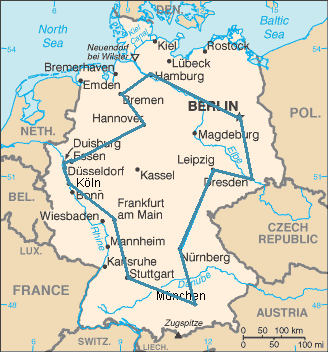
\includegraphics[width=0.5\textwidth]{images/TSP_Deutschland_3.png}
    \caption{\scriptsize{Источник: http://ru.wikipedia.org}}}
  \end{figure}
\end{frame}

\subsection{Условие задачи}
\begin{frame}[fragile]
\frametitle{Задача о коммивояжёре}
	\begin{itemize}
		\item Коммивояжёру для продажи своего барахла нужно посетить несколько городов. Требуется составить кратчайший из возможных путей. Предполагается, что все города соединены прямыми дорогами каждый с каждым.
	\end{itemize}
\end{frame}

\subsection{Концепт решения}
\begin{frame}[fragile]
  \frametitle{Концепт решения - жадный выбор}
	\begin{itemize}
		\item Сама задача имеет множество вариантов решений --- от простых до более сложных.
		\item Одно из возможных решений --- жадный алгоритм. 
		\item Принципов жадного выбора может быть несколько.
		\item Возьмём самый простой --- из каждого города будем ехать в самый ближайший по списку из тех, в которых мы ещё не были.
	\end{itemize}
\end{frame}

\subsection{Хранение данных}
\begin{frame}[fragile]
  \frametitle{Концепт решения - хранение данных}
	\begin{itemize}
		\item Во многих задачах стоит вопрос, как хранить данные?
		\item Вопрос 1: как хранить местоположение городов?
		\item Простейший вариант --- в виде двумерного массива городов. Ключи --- номера городов, значения --- две координаты (широта и долгота в оригинале, но мы решаем в плоской задаче, поэтому $x$ и $y$).
		\item Вопрос 2: надо как-то хранить города, в которых мы уже были.
		\item Для этого можно завести булевский одномерный массив длиной в количество городов. Если мы побывали в $i$-ом городе, то делаем $i$-ый элемент этого массива равным \textbf{истине}. По умолчанию выставляем все элементы равными \textbf{лжи}.
	\end{itemize}
\end{frame}

\subsection{Алгоритм}
\begin{frame}[fragile]
  \frametitle{Алгоритм}
	\begin{enumerate}
		\item Напишем функцию, вычисляющую по теореме Пифагора расстояние между двумя городами. На вход --- координаты городов (в виде двух массивов), на выходе --- вещественное число.
		\item Допустим, мы начинаем в точке (0,0). Так как нам надо пройтись на всем $N$ городам, зададим цикл от 0 до $N-1$ (по количеству шагов).
		\item Перед этим заведём две переменные, показывающие наше текущее местоположение.
		\item Вычислим ближайший к нашему текущему местоположению город. Для этого пройдёмся по всем городам, в которых мы ещё не были (циклом, не рассматриваем такие города, у которых булевское значение соответствующего элемента равно истине).
 	\end{enumerate}
\end{frame}

\subsection{Алгоритм 2}
\begin{frame}[fragile]
  \frametitle{Алгоритм}
	\begin{enumerate}
		\setcounter{enumi}{4}
		\item Вычисление ближайшего города похоже на вычисление минимального элемента массива, только с дополнительным условием в виде истинности элемента булевского массива. Расстояние между городами вычисляем с помощью заданной функции.
		\item Вычислив ближайший город, выведем его на экран, как элемент маршрута. Заменим переменные, в которых мы храним текущие координаты.
		\item В булевском массиве напротив соответствующего города поставим флажок ИСТИНА.
		\item Повторяем операцию вплоть до последнего города. Заканчиваем вместе с первым циклом.
 	\end{enumerate}
\end{frame}

\subsection{Задание}
\begin{frame}[fragile]
  \frametitle{Задание}
	\begin{itemize}
		\item Написать программу для решения задачи о коммивояжёре по предложенному алгоритму.
		\item Придумать такое расположение городов, когда предложенный алгоритм работает очень некорректно (не более 6 городов).
		\item (*) Решить задачу в пространственном случае, когда для каждого города хранятся широта и долгота, а расстояния вычисляются на сфере, а не в плоскости.
	\end{itemize}
\end{frame}

\section{References}
\subsection{References}
\begin{frame}[fragile]
  \frametitle{References}
  \begin{itemize}
    \item Все презентации доступны на http://school.smirik.ru!
    \item Вопросы, предложения, д/з: smirik@gmail.com
  \end{itemize}
\end{frame}

\end{document}
